\documentclass[13pt]{amsart}
\usepackage[margin=0.75in]{geometry} % see geometry.pdf on how to lay out the page. There's lots.
\geometry{a4paper} % or letter or a5paper or ... etc
% \geometry{landscape} % rotated page geometry
\usepackage{amsmath}
%\PassOptionsToPackage{pdfpagelabels=false}{hyperref}
%\usepackage[figure,figure*]{hypcap}
\usepackage[dvipsnames]{xcolor} 
\usepackage{graphicx}
\usepackage{float}
\usepackage{subcaption}
\usepackage{url}
%\usepackage[font=small,labelfont=bf]{caption} % Required for specifying captions to tables and figures

% See the ``Article customise'' template for come common customisations

\title{Term Project Proposal}
\author{Troy Raen}
%\date{} % delete this line to display the current date

%%--------------------------------------------------------------------------------------------------------
% MACROS
% \newcommand{\Msun}{\mathrm{M}_{\odot}} % Msun/h
% \newcommand{\hw}[1]{{\color{TealBlue}[HW #1]}}
\newcommand{\Q}[1]{{\color{gray}\textbf{#1}}}
\newcommand{\p}[2]{\vspace{5mm} \textbf{#1: }{\color{gray}\textbf{#2}}}

%--------------------------------------------------------------------------------------------------------
%%% BEGIN DOCUMENT
\begin{document}

\maketitle
%\tableofcontents



\section{Outline}
% Outline of a learning problem you plan to focus on, type of data you have available. Why is the problem important?

It is well established that the light reaching our telescopes from distant galaxies is shifted toward the red end of the spectrum (relative to the frequency it was originally emitted at), and that this shift increases with the galaxy's distance from us. The combined measurements from many galaxies indicate that the universe itself (the space between galaxies) is expanding at a rate that increases with time. The precise calculation of this expansion rate is being pursued and it depends strongly on our ability to make accurate calculations/estimations of the amount by which the light from a distant galaxy is redshifted. (Actually, the calculations of all fundamental quantities in cosmology rely heavily on these redshifts.)

The calculation of the redshift from measurements of light intensity generally depends on being able to find known features in the intensity as a function of frequency. Poor frequency resolution then increases the error on an estimation of the redshift.

There are two ways in which telescopes can take measurements: spectroscopy and photometry. Spectroscopy records information about the amount of light coming in over a wide range of the frequency spectrum, at high resolution. Photometry essentially divides the spectrum into a small number of bins (on the order of 5) and records aggregated information for each bin. Thus photometry is much cheaper to do and so we have more data of this type. However, this low resolution translates into large errors on our estimates of redshift using this data. (A redshift calculated in this way is called a 'photo-z'.)

I have access, through my advisor, to a dataset consisting of simulated, photometric telescope data for $\sim3 \times 10^{6}$ galaxies, with 3 quantities for each photometric bin (measurement of intensity of light, error on the measurement, one other that I do not yet understand). With 6 bins, this gives 24 features total. The dataset also includes the correct redshift for each galaxy.

The simulated data is intended to mimic the data anticipated from the upcoming Large Synoptic Survey Telescope (LSST). LSST will collect data from large volumes of the sky and at rates several orders of magnitude above any other telescope to date. The community is making large efforts towards dealing with data at this scale, and one of these efforts is toward quick and accurate photo-z calculations. Codes using machine learning algorithms are beginning ($\sim$2000) to be used for these calculations.

\textbf{My proposal is to study how the error in photo-z estimates scale with the size of the training set for different algorithms.}




\section{Learning Methods}
% Learning methods you plan to start with for the problem. References to previous work (if any). Please note, it is expected that during the project you will seek and experiment with additional more advanced ML methods based on the ML literature.

I plan to start with 1) a neural network and 2) a regression decision tree and to quickly expand that to a random forest. S\'anchez et al. (2014) review the codes in use at that time. Here I give an (incomplete) list of the types of methods used in those codes:

\begin{itemize}
\item artificial neural networks
\item prediction trees and random forest
\item boosted decision tree
\item relevance vector machine
\item normalized inner product nearest neighbor
\item various Bayesian methods
\end{itemize}

I am particularly interested in the decision tree and Bayesian methods, but will look in to all of these options. With the current efforts, there may also be codes developed more recently that use other methods. I will do a more thorough search of the literature and also consult with my advisor about algorithms that may be particularly important for LSST.


\section{Testing Solutions}
% How do you plan to test you have succeeded to solve the problem. How do you plan to compare the different solutions.

Newman et al. (2019) have done photo-z error analysis on a random forest regression algorithm (see Figure 1), and found that the error scales as $1/N^{0.4}$ where N is the training sample size. The error was expected to go as $1/\sqrt{N}$, so this result was somewhat surprising. They use two estimates of the error, one is a normalized median absolute deviation and the other is a measure of the number of objects with errors greater than 10\%. Photo-z estimates can be wrong by large margins, so this outlier detection is a useful statistic. I plan to use these two measures when comparing algorithms.

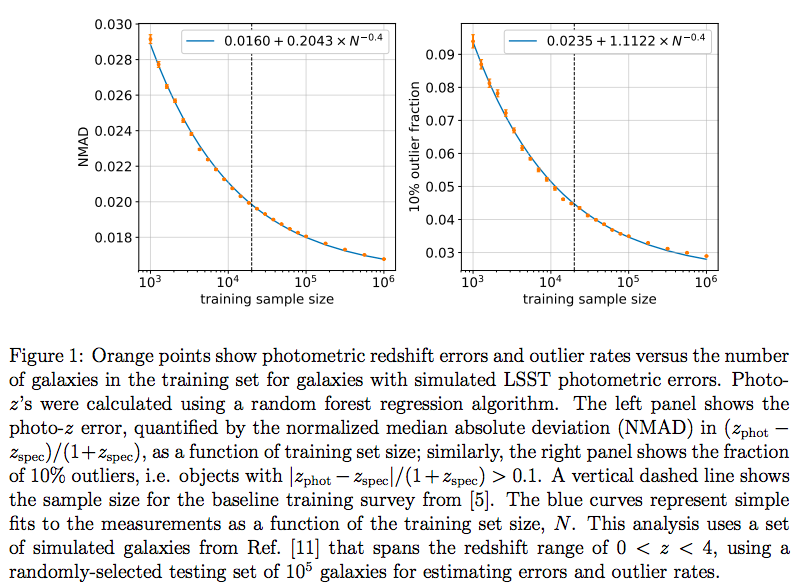
\includegraphics[width=\textwidth]{photozerrors.png}
\captionof{figure}{Reproduced from Newman et al. (2019). Here, $z_{spec}$ is the true redshift.}


\section{Schedule}
% Brief schedule of work (approximate timeline of work)

Tentative deadlines:

\begin{itemize}
\item March 26: neural network
\item April 2: random forest
\item April 9: method 3 (TBD)
\item April 16: method 4 (TBD)
\item April 25: write report
\end{itemize}




\section{References}
Newman et al. 2019 (in prep. scheduled to be posted to the arXiv on March 21, 2019)

S\'anchez et al., Monthly Notices of the Royal Astronomical Society, 1482?1506 (2014)



 


\end{document}
